\documentclass{beamer}

%style
\mode<presentation>
\usetheme{Boadilla}

%Packages
\usepackage[utf8]{inputenc}
\usepackage[ngerman]{babel}
\usepackage{graphicx}
\usepackage{booktabs}
\usepackage{mathtools}
\usepackage{amsmath}
\usepackage{listings}
\usepackage[utf8]{inputenc}
\usepackage[ngerman]{babel}
\usepackage[T1]{fontenc}
\usepackage{lmodern}
\usepackage{tabto}
\usepackage{listings}
%bibtex
\usepackage[backend=biber, style=authoryear]{biblatex}
\addbibresource{referenzen.bib}

%Einstellungen der Präsentation
\title[Cybersecurity]{Flubot:\\ Android-Malware verbreitet sich über Fake-Patches}
\author{Moritz Rupp}
\institute[MR]{Hochschule Albstadt-Sigmaringen}

\date{tobedated - WS 21/22}

%Beginn der Präsentation
\begin{document}

%Titelseite
\begin{frame}
\titlepage
\end{frame}
%Inhaltsverzeichnis
\begin{frame}
\frametitle{Inhalt}
\tableofcontents    
\end{frame}
\begin{frame}{Leitartikel}
\begin{center}
 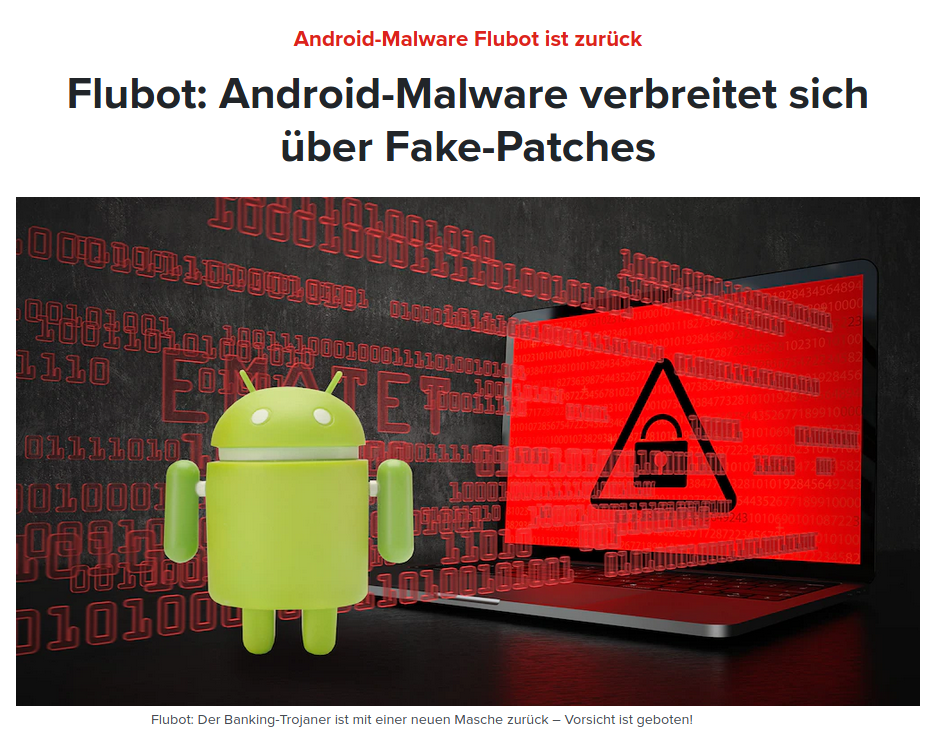
\includegraphics[scale=0.31]{bild.png} 

\end{center}

\end{frame}

\begin{frame}{Trivia}
 \section{Trivia}
 \begin{itemize}
  \item Banking Trojaner - Phishing Malware
  \item Erstes Auftreten Ende 2020 in Spanien\\
  	- Frühjar 2021 in Deutschland
  \item 80 tausend Infizierte Geräte
  \item im Umlauf
  \item Schaden in höhe von 10 Mio €
 \end{itemize}
\end{frame}
\begin{frame}{Was ist Flubot genau?}
- Verbreitung über SMS \\
- kurzer Text mit Link\\
- vermeintlicher Dienst Voicemail etc. \\
- Nur durch herunterladen der apk nutzbar\\

\begin{block}{Banking Trojaner}
 Vermeintlich harmlose Anwendung dringt in System ein und\\
 greift Daten ab.\\
 - In diesem Fall Banking Apps
\end{block}
\begin{block}{Botnetze}
 Große Anzahl an Infizierten Geräten die automatisiert Malware betreiben und sich verbreiten
\end{block}

\end{frame}
\begin{frame}{Funktionsweiße}

\end{frame}

\begin{frame}{Verbreitung}
 Verteilung... \\
 Infection ... \\
\end{frame}
\begin{frame}{Technische Analyse}
In Java geschrieben

\end{frame}
\end{document}
